\section{Introduction}

\subsection{About this document}
This is a document with suspension commissioning tasks described in detail, as in mathematical/theoretical/code/ procedure details.
We sincerely hope that this document can serve as a handbook/guideline for suspension commissioning, and as an educational document for people, who want/need to participate in suspension commission activities, to know more about the activities.

This document is dynamic, and it should be, as we get input and suggestions from people, and as technology evolves.
With that said, if you have an opinion on particular tasks or methods described in this document or suspension commissioning in general, feel free to submit an issue \href{https://github.com/gw-vis/vis-commissioning-tex/issues}{here}.
Alternatively, you can contact the maintainer (Terrence for now) via any communication channels (emails, slack, whatever).
We will update the document accordingly.

As we all know, people have taken different approaches for suspensions commissioning in the past.
And, there were not enough communications between subgroups/people on how suspensions should be configured.
With this repository, we hope to create an open environment for people to exchange ideas regarding suspension commissioning.
And, we wish the document to be filled with ideas and methods that we all agree on, so all of us will commit to follow this document when participating commissioning activities.


\subsection{Suspension commissioning as a stepping stone}
Suspension commissioning is about a series of tasks that get us from hardware installation/upgrade to interferometer commissioning.
In other words, we do whatever is necessary to the suspensions into a state where interferometer commissioners can ``use'' the suspensions to do interferometer alignment and locking, without tweaking the internals of the suspension systems.
With that said, we should have certain expectation on the initial state of the suspension (as hardware teams handover the suspensions to us), and interferometer commissioning team should expect something from us.
So, this document is about defining those expectations and how do we achieve them.

\subsubsection{Hardware expectations}
Before we start working on anything, the suspensions have to be ready for commissioning.
That is, we shouldn't be tweaking the hardware of the suspensions
All tasks that needed to be done at the hardware level, is by definition, not our tasks.
We should expect the suspensions to be ``healthy'', as in, the dynamics of the suspensions are exactly what one would expect, and the sensors and actuators should be fully functional and calibrated.
At the end of the hardware installation process, there's an acceptance test, which every suspension should pass.
This should, in principle, make sure that the suspensions are ``ready''.
But, if we observe anything out of the normal, we should check the system's vitals and explain what's wrong to hardware experts.

There are many ways that hardware fault can leave you head-scratching for a long period of time.
And, sometimes they can be hard to catch, especially when there's no testing pipeline in KAGRA.
I learnt this from painful experience.
I was asked to work on the optical lever on the signal recycling mirror (SR) suspensions.
In particular, I was working on something we called ``diagonalization'' where we align the sensor signals to some desirable basis.
I worked out the math but I can't seem to get the signals decoupled, regardless of the fact that the same method worked for other optical lever.
At the end, we discovered that one sensor (QPD segment) has a higher gain than the others and that was simple a hardware fault that has haunted me and the Type-B team for months \cite{SR2_oplev_diagonalization, Comment_SR2_oplev}.
Also, there's nothing that prevents the suspensions to go "unhealthy" even if it was perfectly fine.
Systems can degrade and degradation can happen.
For example, one of the PRM magnet came off during commissioning \cite{PRM_magnet_came_off, MICH_got_locked}.
Fortunately, commissioners were able to pin point the source of error and asked the vibration isolation system (VIS) team to check it.
The lesson learnt here, is that, we shouldn't trust what was given to us, even if the suspensions were given to us by Albert Einstein himself.
People make mistakes, and there's no exception.
We are scientist, and we need to be skeptical\footnote{If there's anything I (Terrence) learnt from Rana, it's this.}.
So, think carefully if any abnormality is due to hardware fault.
And, do consult hardware experts and demand a hardware fix when you got stuck.

Here is a non-exhaustive list of problems that I can think of\footnote{Please submit an issue if you can think of more that are worth mentioning.}, that can only be fixed at a hardware level, but can limit the outcome of suspension commissioning, and demand fixes:
\begin{itemize}
	\item Suspension in contact with components near it (e.g. Touching a cable). This will usually result in a very low Q-factor in certain vibration modes.
	\item Sensor not within good operation range. This will pose a limit in the amount of actuation during feedback control. This can also result in wrong sensors/actuator diagonalization. And, this can lead to higher sensor noise.
	\item Stepper motors stuck. Static load on actuators cannot be offloaded to stepper motors and hence limiting the actuation force during feedback control.
	\item Suspension cannot be moved in full range (e.g. the BF stage of the SRM \cite{SRM_work}).
	\item Abnormal coupling (e.g. Same signal but with phase difference as reported in \cite{prequa}).
	\item Very different coil actuation efficiency, indicating a non-functional actuator.
\end{itemize}
Fixing these problems are not within the scope of suspension commissioning.
We are suppose to work with a healthy system so we get maximum potential out of the hardware.
We should ask for a fix, before proceeding.
If it can't be fixed, we should discuss possible limitations and possible workarounds together.

\subsubsection{What should interferometer commissioners expect?}
We cannot guarantee that the outcome of suspension commission are exactly needed for interferometer commissioning.
There are few reasons:
1) There are too many uncertainties.
2) Various topics regarding the suspensions are not well-studied, and are still being researched.
3) There are some performances that cannot be confirmed until we have the interferometers.
And most importantly, 4) We don't exactly know what realistically interferometer commissioning needs, except we can only refer to theoretical studies like \cite{Sekiguchi:2016bmv}, which can be outdated and not really aligned with the real deal here in KAGRA.
Therefore, regarding the last point, we strongly encourage interferometer commissioners to cooperate by sharing information and suggestions.

In particular, these information will be very useful:
\begin{itemize}
	\item What is the realistic displacement level requirement, in RMS and peak, for the optics?
	\item At what optics displacement level did you observe lock-loss?
	\item At what seismic noise level did lock-loss occur?
	\item Is lock-loss correlated with the seismic noise level?
	\item How would you like to control the suspensions?
	\item What are the entry points? Do you want to control the suspensions directly from the setpoints? Or do you want to control the suspension using directly from the actuation signals?
	\item Why did you run into actuation saturation? Do you want the signals to be offloaded to higher stages, like the preisolator?
	\item What are some problematic cross-couplings (e.g. length-to-pitch), and in what condition you would like them to be decoupled?
\end{itemize}

While we cannot provide any guarantee, we can and should provide warranty.
If the suspensions are failing, it is suspension commissioners' job to fix or improve it.
Interferometer commissioners should \textbf{not} be tackling suspension tasks like, internal damping of the resonances, sensors decoupling, or seismic noise attenuation.
And, interferometer commissioners should expect the suspensions to behave like a blackbox (as you don't need to know what's happening internally), and as some sort of servo (as it steers the optics).
If the suspensions become problematic and is hindering interferometer commissioning, interferometer commissioners should work with suspension commissioners to tackle the problem.
Previously, such kind of interface was clearly lacking\footnote{As Nakano-san is a superman who tackles every problem on his own.} and we hope this can be improved in the future.
We need good communication for KAGRA to work.
So, here we should say that \textbf{suspension commissioning is not a ``once done and for all'' process}.
Instead, it is something that should be recursively done, as we get ``complaints'' from interferometer commissioners during interferometer commissioning.


\subsection{Goal}
Qualitatively speaking, the goal of suspension commissioning is simply to bring the suspensions into a state where interferometer commissioners can use the suspensions, via defined entry points, to steer the mirrors and make an interferometer, which is sensitive enough to be a gravitational wave detectors.
Althrough, as mentioned, there's no realistic requirements, which are derived from previous experience, we adopt theoretical requirements derived from \cite{Sekiguchi:2016bmv}. In particular, in order for KAGRA to function as an gravitational wave detector, the suspensions have to satisfied 2 types of requirements, displacement noise requirement, residual motion requirement.
In this section, we will briefly discuss the requirements, but will not go into the details, as this is not the scope of this document.
Readers are recommended to refer to the external references cited.

\subsubsection{Displacement noise requirement}
Ground-based gravitational wave detectors have a detection band starting from $10~\mathrm{Hz}$.
The detectable effect of gravitational waves comes in the form of strain, which loosely speaking, is the fractional change in length.
To detect gravitational waves, we simply use an L-shape interferometer and measure the change in the arm lengths in two directions.
We expect targeted gravitational waves to have a peak amplitude of $10^{-21}$.
While the arm lengths of the interferometer are in the order of $10^{3}~\mathrm{m}$, the change in arm lengths caused by targeted gravitational wave is expected to be in the order of $10^{-21}\times 10^{3}~\mathrm{m}=10^{-18}~\mathrm{m}$, which is a very tiny amount of displacement.
Effectively, this means that the test masses (TM), i.e. the end mirrors, must have a displacement level lower than that.
Giving a safety factor of $10$, i.e. signal-to-noise ratio of around 100, this converts a displacement noise requirement of $10^{-19}~\mathrm{m}$ at $10~\mathrm{Hz}$, roughly speaking. Figure.~\ref{fig:displacementnoiserequirement} shows the displacement noise requirement of the optics including the test mass (TM), beamsplitter (BS), signal recycling mirror (SRM), and power recycling mirror (PRM) above $10~\mathrm{Hz}$.
\begin{figure}[!h]
	\centering
	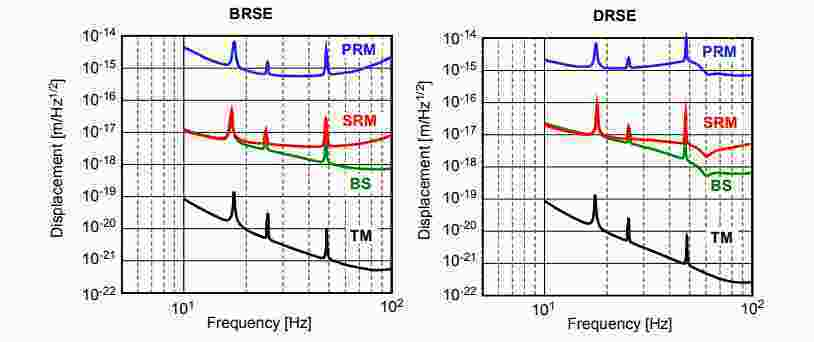
\includegraphics[width=0.7\linewidth]{figures/displacement_noise_requirement}
	\caption{Displacement noise requirements of the test mass (TM) (black), beamsplitter (BS) (green), signal recycling mirror (SRM) (red), and power recycling mirror (PRM) (blue), under boardband resonant sideband extraction configuration (BRSE) (Left) and detuned resonant sideband extraction scheme (DRSE) (Right). Retrieved from \cite{Sekiguchi:2016bmv}.}
	\label{fig:displacementnoiserequirement}
\end{figure}
As can be seen, the requirements of optics other than the TMs are much lower.
The displacement noise level of the BS and the SRM is at $10^{-17}~\mathrm{m}$, while that of the PRM is at $10^{-15}~\mathrm{m}$.
Table~.\ref{table:displacement_noise_requirement} summarizes the displacement noise of various optics at $10~\mathrm{Hz}$.
Therefore, the partial goal of suspension commissioning is to make sure these displacement noise levels requirement are met.
\begin{table}[!h]
	\centering
	\begin{tabular}{|c|c|}
		\hline
		& Displacement level ($\mathrm{m}/\sqrt{\mathrm{Hz}}$)\\
		\hline
		TM &  $1\times 10^{-19}$\\
		\hline
		BS &  $1\times 10^{-17}$\\
		\hline
		PRM & $2\times 10^{-15}$\\
		\hline
		PR2, PR3 & $1\times 10^{-15}$\\
		\hline
		SRM & $1\times 10^{-17}$\\
		\hline
		SR2, SR3 & $5\times 10^{-18}$\\
		\hline
	\end{tabular}
	\caption{Summary of longitudinal displacement noise level (at $10~\mathrm{Hz}$) of the optics including the folder mirrors of the recycling cavity (PR2, PR3, SR2, SR3). Retrieved from \cite{Sekiguchi:2016bmv}.}
	\label{table:displacement_noise_requirement}
\end{table}
The suspensions of the optics are designed specifically to attenuate the seismic noise at $10~\mathrm{Hz}$ to the displacement level specified in table.~\ref{table:displacement_noise_requirement} via passive isolation.
Therefore, the suspensions intrinsically satisfied these requirements already without any tweaking.
However, the main concern here is not about passive isolation.
Instead, it's about active isolation/feedback control, as we need to keep the control noise below these displacement level, while maintaining certain disturbance rejection capability.
This brings us to the other requirement: residual motion.

\subsubsection{Residual motion requirement}
In previous section, we discussed what are the requirements for KAGRA to be sensitive enough to become a gravitational wave detector.
Here, we will discuss the requirements for KAGRA to be an interferometric gravitational wave detector.
In particular, we will discuss velocity, angular fluctuation, and displacement level requirement.
Again, here we only briefly mention the rationale behind such requirements and readers are strongly recommended to read \cite{Sekiguchi:2016bmv} for detailed explanations.

In order for KAGRA to become an interferometric gravitational wave detector, the main optics must be manipulated to form various optical cavities, where feedback control is used to ``lock'' two mirrors at relatively stable separations.
The technique used is called Pound-Drever-Hall (PDH) technique \cite{doi:10.1119/1.1286663}.
To use this technique, the separation between two optics stay within the operating range where the control signal for using PDH technique becomes linear.
In \cite{Sekiguchi:2016bmv}, a velocity requirement of the is derived by considering the maximum actuation power of the TM coils.
Consider a case where the optics are moving towards the operating range.
As the optics enter the range, the actuators applies maximum force on the optics, causing the optics to decelerate maximally.
If the optics are put to halt before they exit the operating range, then lock-acquisition is achieved.
This only happens when the velocity of the optics is lower than a certain threshold, which we define as a requirement.
The velocity requirements the main optics are derived in \cite{Sekiguchi:2016bmv} and is summarized in table.~\ref{table:velocity_requirement}.
\begin{table}[!h]
	\centering
	\begin{tabular}{|c|c|}
		\hline
		& Velocity requirement (RMS) ($\mu\mathrm{m}/\mathrm{s}$)\\
		\hline
		TM, BS, SR &  $0.5$\\
		\hline
		PR &  $2$\\
		\hline
	\end{tabular}
	\caption{Summary of main optics' velocity requirement}
	\label{table:velocity_requirement}
\end{table}

Now, I don't really understand the rationale behind these angular fluctuation requirements\footnote{Please help me to write this section if you know the correction explanation. As far as I know, the angular fluctuation requirement comes from the fact that the interferometer needs to be aligned and that the beam spots are within good range around the center of the optics. But, I don't really know how people got those numbers.} and it seems that different sources suggests different things. I will simply report the requirements from some sources. 

In \cite{Sekiguchi:2016bmv}, it was reported that the RMS angles of the mirrors should not produce beam spot fluctuation on the optics by larger than an RMS value of $1~\mathrm{mm}$.
Using the beam paths as the lever arm, the angle fluctuation requirements are calculated and shown in table.~\ref{table:angular_fluctuation_requirement}.
\begin{table}[!h]
	\centering
	\begin{tabular}{|c|c|}
		\hline
		& Angular fluctuation RMS ($\mu\mathrm{rad}$)\\
		\hline
		TM &  $0.2$\cite{Sekiguchi:2016bmv, yuta_oplev}~/~$0.01$\cite{PhysRevD.88.043007, Mueller:05}\\
		\hline
		BS &  $4$\\
		\hline
		PRM & $45$\\
		\hline
		PR2 & $20$\\ 
		\hline
		PR3 & $2$\\
		\hline
		SRM & $25$\\
		\hline
		SR2 & $10$\\
		\hline
		SR3 & $1$\\
		\hline
	\end{tabular}
	\caption{Angular fluctuation requirements of the optics. Retrieved from \cite{Sekiguchi:2016bmv, yuta_oplev} unless otherwise specified.}
	\label{table:angular_fluctuation_requirement}
\end{table}

However, in another source regarding beam jittering at LIGO \cite{Mueller:05}, it's mentioned that the angular fluctuation requirement of the test masses at LIGO is $10^{-8}~\mathrm{rad}$.
The same value is also used to derive the wavefront sensor sensitivity requirement at KAGRA \cite{PhysRevD.88.043007}.
It's worth noting that both of these sources were also cited in \cite{Sekiguchi:2016bmv}.
So unless there's extra comment regarding this, let's just set the requirement for the TM to the lower one ($10^{-8}~\mathrm{rad}$) as a worst case scenario\footnote{There's a chance that we cannot confirm that we actually satisfied this requirement at the end of suspension commissioning as there's no sensors sensitive enough to measure such small level of fluctuation.Let's hope that our optical levers are sensitive enough}.

At last, the longitudinal displacement requirement was derived also from the maximum actuation power of the force coils at the TM stage.
Doing so, we assume that only these actuators are used during lock acquisition, but this may not be the case, so here again we are assuming a worst case scenario.
Table.~\ref{table:displacement_rms_requirement} summarizes the displacement RMS value requirement of the main optics in KAGRA.

\begin{table}[!h]
	\centering
	\begin{tabular}{|c|c|}
		\hline
		& Displacement RMS requirement ($\mu\mathrm{m}$)\\
		\hline
		TM &  $0.01$\\
		\hline
		BS &  $3.3$\\
		\hline
		SRM & $3.3$\\
		\hline
		SR2, SR3 & $1.6$\\
		\hline
		PRM & $560$\\
		\hline
		PR2, PR3 & $280$\\
		\hline
	\end{tabular}
	\caption{Longitudinal displacement RMS requirement of the optics. Retrieved from \cite{Sekiguchi:2016bmv}.}
	\label{table:displacement_rms_requirement}
\end{table}

This concludes the residual motion requirements for the core optics. 
So, the other half of the goal is to actively control the suspensions so requirements as shown in Table.~\ref{table:velocity_requirement}, \ref{table:angular_fluctuation_requirement}, and \ref{table:displacement_rms_requirement} are met, while not violating noise specification as shown in Table.~\ref{table:displacement_noise_requirement}.
In the following sections, we shall discuss/review some of the methods and techniques that can be used to achieve these goals.
We will also discuss some ways that we used to verify the satisfaction these requirements.

\subsubsection{Miscellaneous requirements}
Guardian
90th seismic noise





